\documentclass[pdftex,a4paper,titlepage,11pt]{article}

% Les packages de base pour le support du français
\usepackage[utf8]{inputenc}
\usepackage[T1]{fontenc}
\usepackage[english]{babel}

% La bonne police, sans serif, helvetica
\usepackage[scaled]{helvet}
\renewcommand*\familydefault{\sfdefault}
% \usepackage{palatino} % Palatino font
% \usepackage{lucidabr}

% Pour les liens/urls
\usepackage[colorlinks=true,linkcolor=black,citecolor=black,urlcolor=black,filecolor=black]{hyperref}

% Le reste
\usepackage{verbatim}
\usepackage{graphicx}

% Pour ne pas avoir à mettre images/ devant les noms d'images...
\graphicspath{{images/}}
\usepackage{fullpage}
\usepackage{array}
\usepackage[absolute]{textpos}
\usepackage{framed}

% Pour les entêtes et les pieds de page
\usepackage{fancyhdr}
\pagestyle{fancy}
\usepackage{fancybox}

\usepackage{lastpage}
\usepackage{datetime}
\usepackage{multicol}
\usepackage{multirow}
\usepackage{eso-pic}
\usepackage{color}
\usepackage{sectsty}

% Pour avoir de beau listings
\usepackage{listings}
\usepackage{color}
\usepackage{textcomp}
\definecolor{listinggray}{gray}{0.9}
\definecolor{lbcolor}{rgb}{1,1,1}
\lstset{
	backgroundcolor=\color{lbcolor},
	tabsize=4,
	rulecolor=,
% 	language=bash,
	upquote=true,
	aboveskip={1.5\baselineskip},
	columns=fixed,
	showstringspaces=false,
	extendedchars=true,
	breaklines=true,
	prebreak = \raisebox{0ex}[0ex][0ex]{\ensuremath{\hookleftarrow}},
	frame=single,
	showtabs=false,
	showspaces=false,
	showstringspaces=false,
	identifierstyle=\ttfamily,
	keywordstyle=\color[rgb]{0,0,1},
	commentstyle=\color[rgb]{0.133,0.545,0.133},
	stringstyle=\color[rgb]{0.627,0.126,0.941},
}

\addtolength{\voffset}{-20pt}
\addtolength{\topmargin}{-6pt}
\addtolength{\headsep}{+12pt}
\addtolength{\footskip}{-4pt}
\addtolength{\textheight}{-23pt}
% \usepackage[top=1.5cm, bottom=5.5cm, left=2.5cm, right=2.5cm]{geometry}

% Pour le glossaire
% \usepackage[xindy, toc]{glossaries}
\usepackage[french]{nomencl}


%%Redefinition de commandes et autres utilitaires

%Ecart entre les colonnes
% \setlength{\columnseprule}{0.5pt}

% Définition des couleurs de l'ENSIB
\definecolor{darkBlueENSIB}{RGB}{0,52,120}
\definecolor{lightBlueENSIB}{RGB}{0,152,195}

\definecolor{fushiaENSIB}{RGB}{203,0,68}
\definecolor{orangeENSIB}{RGB}{255,109,34}

%Changement des couleurs des titres
\partfont{\color{darkBlueENSIB}{}}
\chapterfont{\color{darkBlueENSIB}{}}
\sectionfont{\color{darkBlueENSIB}{}\huge}
\subsectionfont{\color{darkBlueENSIB}{}\Large}
\subsubsectionfont{\color{darkBlueENSIB}{}\large}

\makeindex
% \makeglossaries
\makenomenclature

%Derniere page avec queue du poisson
\newcommand{\lastPage}{
	\newpage
	\strut
	\fancyhf{}
	\renewcommand{\headrulewidth}{0pt}
	\addtocounter{page}{-1}
% 	\AddToShipoutPicture*{\BackgroundPic{atos-logo-light.png}}
	\AddToShipoutPicture*{\BackgroundPic{Tux_n&b_half_1.png}}
	\newpage
}

% Modification du nom de la table des matières
% Ne semble pas fonctionner
% \renewcommand{\contentsname}{Sommaire}
% Titre pour le Glossaire/Index des noms
\renewcommand{\nomname}{Glossary}
%Separateur des dates
\renewcommand{\dateseparator}{-}

\renewcommand{\title}[1]{
	\vspace*{2cm}
	\begin{center}
		\Huge\textbf{{#1}}
	\end{center}
	\vspace{1cm}
}

\renewcommand{\author}[2]{
	\begin{center}
		\textbf{\Large{#1}}\\
		\normalsize{#2}
	\end{center}
	\vspace{0.3cm}
}

\newcommand{\school}[1]{
	\begin{center}
		\large{#1}
	\end{center}
	\vspace{1.0cm}
}


\newcommand{\supervisor}[4]{
	\begin{center}
		\begin{normalsize}
			{\bf#1}\\
			#2\\
			#3\\
			#4
		\end{normalsize}
	\end{center}
}

\newcommand{\clearemptydoublepage}{
	\newpage{
		\pagestyle{empty}
		\cleardoublepage
	}
}

\newcommand\BackgroundPic[1]{
	\put(0,-100){
		\parbox[b][\paperheight]{\paperwidth}{
			\vfill
			\centering
			\includegraphics[width=\paperwidth, height=\paperheight, keepaspectratio=true]{#1}
			\vfill
		}
	}
}

%%
%% Redefinition des en-tetes et pieds de pages
%%
\fancyhf{}
\fancypagestyle{plain}

%%En tete
\lhead{\hspace{2.3cm}\large \textbf{Integrating PIGA-MAC into the Linux kernel\\}}

% \chead{\large \textbf{Integrating PIGA-MAC into the Linux kernel\\}}

\rhead{
\includegraphics[height=2.1cm, keepaspectratio=true]{Logo_ENSIB.png}}

%%Pied de page
\lfoot{}

\cfoot{\vspace{-0.8cm}\rule[0pt]{\textwidth}{0.1mm}\small \ovalbox{\thepage/\pageref{LastPage}}}

\rfoot{\ddmmyyyydate \today}

%%
%% DOCUMENT
%%

\begin{document}

\begin{titlepage}
%%
%% Page de couverture
%%

\AddToShipoutPicture*{\BackgroundPic{Tux_n&b_half.png}}

\begin{center}
	
\includegraphics[width=6cm, keepaspectratio=true]{Logo_ENSIB.png}
\end{center}

\vspace{0.5cm}

\begin{center}
	\fontsize{30}{30}\selectfont Integrating PIGA-MAC into the Linux kernel\\
	\vspace{2cm}
	\Huge 3rd year STI research project\\
	\Huge 2011 -- 2012
\end{center}

\vspace{2cm}

\begin{center}
	\begin{tabular}{rl}
		\hspace{7.5cm}
		\huge Teacher : & \huge Jérémy Briffaut\\[4pt]
		\huge Student : & \huge Timothée Ravier
	\end{tabular}
\end{center}

\vspace{0.5cm}

\begin{center}
\hspace{7.5cm}
\includegraphics[width=5cm, keepaspectratio=true]{Logo_SELinux.pdf}
\end{center}

\end{titlepage}

\newpage

~\thispagestyle{fancy}

\newpage

~

\vspace{1cm}
\addtocounter{page}{-1}

\section*{Acknowledgments}

~

I would like to particularly thank Jérémy Briffaut for the many advice he gave me. This project is mostly based on his thesis and last years work.

~

I would like to thank Martin Peres for introducing me to the PIGA concept and kernel development.

~

\newpage

\tableofcontents

\newpage

\listoffigures

\newpage

\section*{Introduction} \addcontentsline{toc}{section}{Introduction}

This project is an integral part of my formation at the ENSI de Bourges, a computer science and security french engineering school.

\bigskip

PIGA (Policy Interaction Graph Analysis) is an advanced Mandatory Access Control mechanism designed to enforce security policy on a system. Just like SELinux, PIGA does not directly prevent vulnerability exploitation, but prevents any further action an attacker might attempt to perform on the system.

\bigskip

The current PIGA design faced unexpected problems and some of them are related to the fact that the decision making code is located in userspace. That's the main difficulty that we are trying to address with this kernel port. Among the other problems that I will have to solve, they are multi-core and multi-processor related issues. I will also try to improve performance and ease of use if I succeed in porting the complete PIGA feature set.

\bigskip

I will begin with a short description of all currently available protections for the main open source operating systems such as Linux distributions and some from the BSD family. Then I will proceed to some PIGA reminders, kernel/userspace implementation design. Finally I will compare PIGA-Linux performance to kernel with either nothing, PaX, SELinux, ``classic'' PIGA enabled.

% FIXME

\newpage

\section{State of the art}

\subsection{Context and study limits}

%TODO Add intro

There is a wide range of computer security problems, from hardware specific ones to sotfware related flaws.

\bigskip

In this project, we will not focus on kernel security or kernel hardening (despite the name PIGA-Linux). The main goal of PIGA is to go further than SELinux, in order to enforce security properties on an operating system. So I'll focus my study on mechanisms which allow a user or an administrator to control permissions given to a program running on a computer.

\bigskip

Thus, I will use several restrictions to further constrain this study:
\begin{itemize}
	\item we are limited to the operating system ; we do not take into account interactions with an other system on the network for example ;
	\item we want the solution to be as architecture independant as possible ; we should not require specific hardware design to work properly ;
	\item as we do not take into account the underlying hardware, we do not focus on hardware flaws either and thus do not study hardware based attacks (defective network card or driver...) ;
	\item we should focus on systems which have the source code available for study ;
\end{itemize}

\smallskip

Most of current operating system are using an access control design to ensure minimal security and control on user's activities. The were introduced to limit the effects of an attack against the operating system. But this limited control does not prevent complex attack scenario, such as the compromission of a service which was given adminstrative rights on the system. \cite{NSATIOF} describes in details most of the problems current operating systems are still facing nowadays.

\bigskip

Generally speaking, we lack a global, truly enforced, system wide security mechanism. More than simple checks in interactions between kernel and userspace, it's the whole interaction set on a system that need to be controlled.

\bigskip

First I'm going to detail the objectives an operating system has to achieve. Then I will discuss theorical models and their implementations in modern systems.

\bigskip

In this study, I will refer to files (and others ressources such as sockets) as objects, and to program as subjects, whether or not they are directly controlled by a real human user on the system.

\subsection{Generality}

\subsubsection{Security objectives}

% FIXME find the paper on security objectives
There are three main objectives defined in \cite{SECOBJ}. An operating  system has to provide means to ensure they can be enforced:

\bigskip

\textbf{Confidentiality :}
Information must only be available to users who need it and have the corresponding priviledge. Example: a user should not have access to other users passwords, files or secrets ; classified informations should not be available for unclassified users to read.

\medskip

\textbf{Intégrity :}
The system must remain in coherent state. Example: important informations such as passwords, which programs are installed and their content, configuration files, should not be alterable by unpriviledge users.

\medskip

\textbf{Disponibility :}
The system must remain stable, reactive and usable. Programs have to function properly. Added security controls should limit as little as possible legitimate system functionnality and programs.

\bigskip

Other properties (authenticity...) can be defined as derivatives, as explained in \cite{THESEBRIFFAUT}. Examples:
\begin{itemize}
	\item priviledge abuse: ...
	\item ... % FIXME
\end{itemize}

\smallskip

I will focus on the first two properties, which are confidentiality and integrity. Attack scenario such as Denial of Service will therefore not be taken into account as their goal is to limit a system disponibility. Futur references to security objectives will include only those two.

\bigskip

However, a security solution should not turn a working system to an unsable one and thus can not have a high footprint on ressources. I'll try to limit the impact on performance of the chosen solution.

\subsubsection{The principle of least privilege}

Une des techniques les plus couramment utilisées pour tenter d'atteindre ces objectifs consiste à appliquer le principe de séparation des privilèges ou principe de moindre privilège. Il stipule qu'un programme (contrôlé ou non par l'utilisateur) ne doit disposer que des droits strictement nécessaires à son bon fonctionnement.

\bigskip

Par exemple, un logiciel de traitement de texte n'a pas besoin d'avoir accès aux informations sensibles du système comme la liste des utilisateurs ou la liste des mots de passe.

\bigskip

Tous les principaux systèmes d'exploitation actuels disposent maintenant de mécanismes mettant en place la séparation des privilèges. L'application la plus courante de ce principe est la séparation entre les différents comptes sur un système. Une application lancée par un utilisateur ne bénéficie que des droits accordés à cet utilisateur.

\bigskip

Il faut cependant noter que ce principe ne constitue pas une démarche exhaustive permettant d'assurer des objectifs de sécurité.

\subsubsection{Who/what do I need to trust?}

Il est possible d'employer différentes approches pour s'assurer de la sécurité d'un système d'exploitation, mais chacune d'entre elles repose à un moment ou un autre sur la confiance que l'on a dans l'un des éléments qui la constitue. On distingue ainsi plusieurs situations \cite{WCS}:

\begin{itemize}
  \item faire confiance à tous les logiciels à propos du respect de la politique de sécurité, tout en étant conscient que les logiciels ne sont pas de confiance ;% Trust all the software to abide by a security policy but the software is not trustworthy (this is computer insecurity).
  \item faire confiance à tous les logiciels à propos du respect de la politique de sécurité et s'assurer que le logiciel est validé et fiable (analyse complète et exhaustive de tous les cas d'utilisations, de toutes les branches du code) ;% Trust all the software to abide by a security policy and the software is validated as trustworthy (by tedious branch and path analysis for example).
  \item ne faire confiance à aucun programme, mais imposer une politique de sécurité même si la fiabilité de cette politique et son moyen d'application ne sont pas complétement assurés ;% enforce a security policy with mechanisms that are not trustworthy (again this is computer insecurity).
  \item ne faire confiance à aucun programme, mais s'assurer qu'une politique de sécurité est appliquée par des mécanismes matériels de confiance.% trustworthy hardware mechanisms.
\end{itemize}

Les modèles de sécurité standard se situent tous dans la première catégorie alors que les méthodes que nous allons présenter par la suite peuvent être placées dans les catégories trois et quatre. Le test complet de tous les logiciels présents sur un système d'exploitation est une tâche difficilement réalisable si l'on considère la diversité des matériels disponibles et la complexité d'une application telle que le noyau d'un système d'exploitation. Il existe des systèmes d'exploitation et plus particulièrement des noyaux certifiés Critères Communs \cite{CCCERT}, tel QNX\cite{QNX}, qui peuvent être classés dans la catégorie 2. En revanche, le code source de ces différents systèmes n'étant pas disponible librement, nous ne les détaillerons pas dans ce document.

% An example of hardware based integrity control

% \begin{figure}[h]
% 	\centering
% 	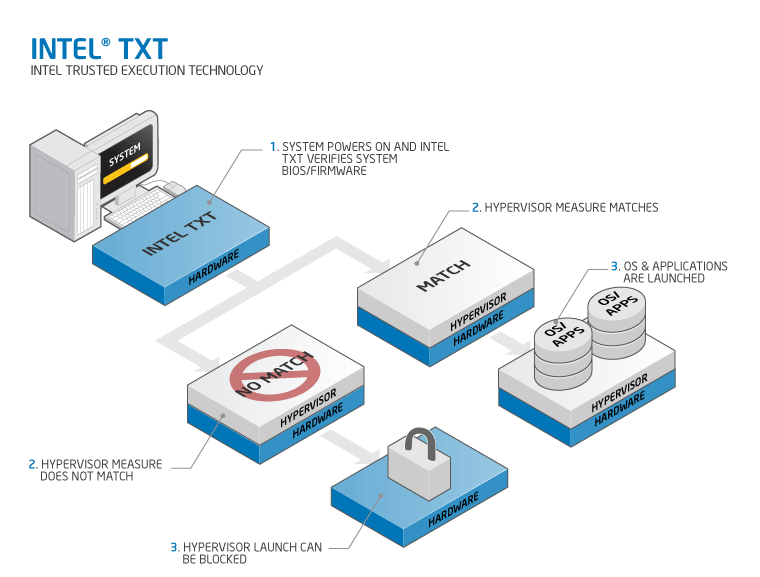
\includegraphics[scale=0.70]{attachements/techrefresh-info-txtfull.png}
% 	\caption{Intel Trusted Execution Technology}
% \end{figure}

\subsection{Les différentes méthodes de contrôle d'accès}

Pour atteindre les objectifs détaillés précédemment et obtenir la séparation et la minimisation des privilèges, les systèmes d'exploitations actuels ont implenté différentes méthodes de contrôle d'accès. Nous allons donc les présenter dans cette partie.

\subsubsection{Discretionary Access Control (DAC)}

Le contrôle d'accès discrétionnaire correspond à un modèle laissant à l'utilisateur, et donc aux programmes, tout contrôle sur les droits accordés aux objets qu'il possède. Un logiciel dispose ainsi la plupart du temps de droits bien superieurs à ces besoins (Firefox a par exemple accès à la liste des comptes utilisateurs). Un sujet (utilisateur ou logiciel) peut ainsi compromettre la confidentialité d'un système en accordant des droits importants à d'autres utilisateurs sur les fichiers qu'il possède. Ce modèle ne permet pas d'assurer la confidentialité, l'intégrité d'un système. Il est à ranger dans la première catégorie des modèles qui font confiance aux logiciels sans imposer de contrôle de sécurité fort.

\subsubsection{Mandatory Access Control (MAC)}

Le contrôle d'accès mandataire repose sur la séparation entre les applications et l'entité prenant la décision d'autoriser ou d'interdire une action. Cette entité peut être implémentée au sein du noyau ou à l'aide de mécanismes externes au système, matériels \cite{ITXT}. Ce modèle permet d'assurer la conformité du système à un ensemble de règles qui forme une politique de sécurité. Il est ainsi possible d'appliquer le principe de moindres privilèges en partant d'une base n'autorisant aucune interaction puis en rajoutant progressivement des interactions autorisées. Le contrôle d'accès mandataire correspond aux catégories trois et quatre, où l'on ne fait pas confiance aux applications pour se reposer sur la mise en \oe{}uvre d'une politique de sécurité plus ou moins fiable.

\subsubsection{Multilevel Security and Multi Categories Security (MLS \& MCS)}

Le modèle de sécurité multiniveau permet d'atteindre certains des buts fixés comme l'intégrité ou la confidentialité. Il repose sur la séparation des objets/sujets en plusieurs domaines, imposant des règles limitant les interactions entre ces mêmes domaines.

\bigskip

\textbf{Bell-LaPaluda :} Ce modèle préserve la confidentialité de l'information en n'autorisant un sujet à écrire uniquement dans un niveau de confidentialité supérieur ou égal, et à ne lire que dans un niveau de sécurité inférieur ou égal. Ce modèle présente plusieurs inconvénients majeurs parce qu'il ne permet pas d'imposer des contraintes d'intégrité et ne permet pas de faire de distinctions précises entre deux personnes possédant le même niveau d'accréditation.

\begin{figure}[h]
	\centering
	\includegraphics[scale=0.5]{bell-lp}
	\caption{Le modèle Bell-LaPadula}
\end{figure}

\bigskip

\textbf{Biba :} A contrario du modèle précédent, c'est l'intégrité qui est préservée, car seules les modifications dans un niveau de sécurité inférieur sont autorisées, et la lecture ne peut se faire que sur un niveau d'intégrité supérieur.

\begin{figure}[h]
	\centering
	\includegraphics[scale=0.5]{biba}
	\caption{Le modèle Biba}
\end{figure}

\bigskip

Les modèles suivant ne peuvent donc se suffirent à eux-mêmes car ils ne permettent pas d'atteindre plus d'un ou deux objectifs à la fois. Ils posent aussi le problème de la sur-classification des données (toutes les données devenues confidentielles), conduisant à l'introduction d'une méthode de dé-classification de l'information, compromettant l'ensemble du modèle.
En pratique, ces modèles peuvent être utilisés sur des ensembles restreints comme nous le verrons par la suite.

\subsubsection{Role Based Access Control (RBAC)}

Plus qu'un modèle réel de contrôle, c'est un modèle d'administration permettant de simplifier le travail de l'administrateur d'un système utilisant un contrôle mandataire. Le principe du contrôle d'accès mandataire consiste à attribuer des rôles à chaque utilisateur de la machine. Ces rôles donnent ainsi accès à différents éléments du système. Par exemple, les rôles d'utilisateur, d'administrateur et de webmestre peuvent être définis et un utilisateur classique pourra se voir attribuer le rôle de webmestre lui autorisant de modifier les pages disponibles sur un serveur sans avoir besoin de donner un accès administrateur complet à cette personne.

\subsubsection{Type Enforcement}

Ce principe repose sur l'association d'un contexte de sécurité à chaque sujet et objet (pocessus, socket, fichier...). L'accès à un object par un sujet doit correspondre à une règle de la politique de sécurité pour être autorisé. Ce modèle nécessite l'attribution d'un contexte de sécurité à tous les objets du système, y compris les fichiers présents sur les supports de stockage.

\subsection{Available solutions to enforce Mandatory Access Control}

Nous allons détailler les implémentations de ces modèles de sécurité dans certains systèmes d'exploitation, notamment les systèmes ``libres'', pour lesquels nous pouvons avoir accès au code source : Linux et la famille des BSD.

\subsubsection{Simplified Mandatory Access Control Kernel (SMACK)}

\subsubsection{TOMOYO Linux}

\subsubsection{Application Armor (AppArmor)}

\subsubsection{Security Enhanced Linux (SELinux)}

SELinux est une implémentation d'un mécanisme de contrôle d'accès mandataire basé sur le ``type enforcement'', de niveaux de sécurité/confidentialité non prédéfinis, et d'un contrôle d'accès basé sur les rôles. SELinux a été développé par la National Security Agency (NSA) et a été intégrée au noyau Linux une fois que l'architecture des Linux Security Modules fut mise en place. SELinux permet de contrôler pour chaque appel système la validité de l'interaction par rapport aux définitions d'une politique. On associe à chaque objets et processus un context de sécurité. L'accès à un object par un processus doit correspondre à une règle de la politique SELinux pour être autorisé. Il faut noter que chaque décision est prise indépendamment des précédentes : SELinux n'as pas de mémoire des transitions effectuées sur un système. C'est cette limitation et la possibilité d'utiliser les flux d'informations indirects, donc non contrôlés par SELinux, qui ont poussé la création de PIGA.

\begin{list}{}{}
 \item \textbf{Contrainte pour l'administrateur :} Il faut décrire la totalité des interactions possibles pour chaque programme présent sur un système. Il faut s'assurer du bon fonctionnement de ces politiques. Il n'existe pas d'outils pour valider les politiques SELinux. Seuls certains systèmes de fichiers supportent les attributs étendus nécessaires à la labelisation des fichiers présents sur les supports de stockage.
 \item \textbf{Avantages :} Séparation fine des privilèges et des rôles, intégrée dans le noyau. Des politiques ont déjà été écrites. Il existe une distribution facilitant le déploiement de ce type de protection : Fedora.
\end{list}

\subsubsection{Policy Graph Interaction Analysis - Mandatory Access Control (PIGA-MAC)}

L'ensemble désigné sous le nom de PIGA est le résultat de la thèse de Jérémy Briffaut ainsi que des contributions de l'équipe SDS du LIFO, et des étudiants de l'ENSIB. Il est constitué notamment d'une sur-couche à SELinux permettant de définir et imposer des propriétés de sécurité à l'échelle du système en plus des contrôles au niveau des interactions effectués par SELinux. Il apporte une ``mémoire'' à SELinux. Un tel résultat est obtenu après génération du graphe complet des interactions possibles et autorisées par une politique SELinux, recherche de chemins interdits, et consignation de ces chemins. Cette solution permet un contrôle plus avancé sur les flux d'informations dans un système, qu'ils soient directs ou indirects.

\begin{list}{}{}
 \item \textbf{Contrainte pour l'administrateur :} Connaissance du langage de définition de propriété PIGA, maîtrise préalable de SELinux, pré-requis matériels pour la ``compilation'' des politiques.
 \item \textbf{Avantages :} Un contrôle très fin sur les interactions dans un système, restriction (statique) des privilèges maximale.
\end{list}

Le système d'exploitation PIGA-OS basé sur la recherche effectuée sur PIGA a été vainqueur du concours Sec\&Si organisé par l'Agence Nationale pour la Recherche (ANR) \cite{PIGASAINTMALO}\cite{PIGAPROP}.

\subsubsection{PaX \& grsecurity}

grsecurity est une autre implémentation des mécanismes de contrôle d'accès mandataire et des listes de contrôle d'accès. Il permet aussi une gestion des droits basée sur les rôles. Souvent associé à \textsc{grsecurity}, PaX est un patch pour le noyau Linux ajoutant des restrictions et des contrôles sur les accès à la mémoire.

\begin{list}{}{}
 \item \textbf{Contrainte pour l'administrateur :} Certains programmes ne fonctionnent plus avec les restrictions implémentées par PaX. Il faut organiser correctement les binaires car la labellisation est effectuée par rapport à l'arborescence
 \item \textbf{Avantages :} Protection avancée de l'utilisation de la mémoire avec PaX (pile non exécutable, ...), fonctionnement un peu plus simple que SELinux
\end{list}

\subsubsection{W\^{}X \& TrustedBSD}

Présentation de W\^{}X.

Le projet TrustedBSD consiste à intégrer à FreeBSD des fonctions de sécurité telles que les attributs étendus pour le système de fichier UFS2, les listes de contrôle d'accès, des capacités d'audit liées à la sécurité, plusieurs méthodes de contrôles d'accès mandataire.

% \subsubsection{PIGA-SYSTRANS ou contextd}
%
% Contextd est un démon chargé de coordonner différents mécanismes de sécurité sur un système Linux. En effet, dans toutes les solutions décrites précédemment, les programmes se voyaient attribuer les droits dont ils avaient besoin, pour toujours. Une application utilisant ponctuellement le réseau se voyait attribuée le droit définitif d'utiliser un port. Contextd introduit la notion de domaine (web, impôts, ...) lié à une activité particulière de l'utilisateur. Les programmes surveillés n'ont le droit de faire que ce qui leur est autorisé dans le domaine courant.
% \begin{list}{}{}
%  \item \textbf{Contrainte pour l'administrateur :} Maîtrise de SELinux, PIGA. Rédaction et test des règles exhaustives pour faire fonctionner les programmes avec contextd. Certains programmes nécessitent des modifications, surtout lorsque ceux-ci ont un comportement inter-domaine.
%  \item \textbf{Avantages :} Presque la plus fine implémentation du principe de moindre privilèges.
% \end{list}

% Pax = sécurité automatique
% SELinux, GrSec = MAC qui contrôle les accès directs
% PIGA = contrôle les accès indirects
% iptables contrôle le trafic réseau
%
% contextd = chef d'orchestre + changement dynamique des règles des autres  mécanismes de protection pour adapter les permissions au domaine d'utilisation.
%
% Chercher tous les systèmes de MAC/DAC/RBAC,...
%
% Classer les MAC en fonction du travail à faire par l'administrateur ? en fonction d'où ils agissent ? par rapport à la logique interne (stateless ou statefull) ?

\newpage

\section{Development and test environment}

PIGA features are intrinsically link to SELinux features so the choice of development environment was limited. The main GNU/Linux distributions supporting SELinux are :

\begin{itemize}
	\item Red Hat Enterprise Linux \cite{RHEL}, CentOS \cite{CENTOS}, Scientific Linux \cite{SL}, Fedora \cite{FEDORA}
	\item Gentoo \cite{GENTOO} with the Hardened Gentoo project \cite{GENTOOH}
\end{itemize}

As PIGA-OS is based on Hardened Gentoo, I chose to stick with this distribution.

\subsection{Hardened Gentoo}

The Hardened Gentoo Project has taken upon the goal of building a completly secure operating system from the ground up. To achieve this goal, several particularities have been selected :
\begin{itemize}
	\item a linux kernel with the PaX \& grsecurity patch
	\item a carefully crafted une configuration and several restrictive compilation options
	\item a modular SELinux policy
\end{itemize}

The first step of this project was to setup a virtual Hardened Gentoo development environment.

The Gentoo choice was also driven by the fact that I had to understand most of the building process in order to make it work properly. This constrain was actualy a benefit.

\subsection{QEMU, KVM and the Virtual Machine Manager}

In order to ease the development process, I used some KVM and QEMU special features. QEMU enabled me to use an externaly (as in: not on a virtual drive) compiled kernel. I saved a lot of time compiling kernels on the host system instead of the virtual one. As the host and the virtual machine architecture matchs (x86\_64, no cross-compilation involved) I was able to use this kernel into a Gentoo virtual machine.

% FIXME
% \subsection{Related tests}

% This virtual environment allowed me to test several of the available solutions (SMACK, TOMOYO...).
% J'ai ainsi créé une machine virtuelle pour chaque solution et j'ai testé les scénarios d'attaques et la réponse que pouvait apporter un administrateur à ces scénarios.
% Violation d'intégrité :
% Violation de confidentialité :
% \subsection{Résultats}
% Tableau comparatif avec le DAC...

\newpage

\section{PIGA-Linux}

\subsection{Objectives}

The following objectives (and implementation order) were layed out with Jérémy Briffaut at the begining of the project :

\begin{enumerate}
	\item Implement a basic decision making algorithm in the kernel
	\item Create userspace tools to load a PIGA policy into the kernel
	\item Optimize the policy storage into the kernel to handle large policy (more than three hundred thousand signatures) in order to make this usefull in the real world
	\item Implement remaining PIGA-IDS and PIGA-IPS fonctionnality (conditionnal policy, process based signatures, better audit features, rule learning, state save and restore...)
\end{enumerate}

\subsection{Architecture}

PIGA-Linux is divided between a kernel patch, a userspace tool, and ``standard'' PIGA tools. This project focused only on the kernel patch and the policy loader tool. The ``standard'' tools functionnality will be briefly explained here for convenience.

\subsubsection{PIGA tools}

%FIXME
Tools to generate graphs and policy files from SELinux policy files. IDS and IPS Java stuff. Original kernel patch description.

\subsubsection{Linux kernel implementation}

As of today, the kernel implementation is severly limited in terms of performance, but fullfils the basic purpose of PIGA.

% Implementation details

It is also as least intrusive as possible as only two major files need minor modifications. The decision taking algorithm for SELinux regroups every checks in a single function, allowing us to easily add the PIGA control after the SELinux one.
As all SELinux behaviours remain unchanged, PIGA denials currently appear as SELinux denials. For now, we can keep the SELinux auditing interface to audit PIGA denials. In future development, we should include a flag or a special field specifying that this particular denial is related to PIGA.

% Séparer les lectures des écritures d'états des signatures pour faire avancer les signutures.

\subsubsection{Piga Policy Parser}

The PIGA Policy Parser (PPP) is a userspace tool built with Flex and Bison (the GNU Lex \& Yacc equivalent). It parses and checks the correctness of a set of signatures contained in a policy file. Those signatures were previously generated with PIGA related tools from a set of PIGA rules and a SELinux policy.

The PPP currently offers very basic features and options :
\begin{itemize}
	\item -h: prints the help
	\item -v: turn verbose mode on, printing warnings for secrity contexts found in the PIGA policy but not in the loaded SELinux policy
	\item -s: display some statistics from the PIGA policy, such as the count of each security context
	\item NOT IMPLEMENTED YET :
	\item -e: enable PIGA once if the policy loaded successfully
	\item -n: do not enable PIGA after loading the policy (default)
	\item -l: load the given SELinux module before loading the PIGA policy
	\item -f: use full check mode for PIGA
	\item -a: use SELinux audit mode for PIGA (requires a custom SELinux module which can be loaded with -l)
	\item -r: restore previous PIGA state using designated file
	\item -c: enable conditionnal signatures (PIGA feature not yet available)
	\item -w: enable warning mode (PIGA feature not yet available)
\end{itemize}

\smallskip

In order to load a policy into the kernel, you need to give a policy file to the tool standard input (classic input from a file as an argument will be implemented: ppp [-hvsenfacw] [-l selinux\_module] < PIGA\_policy.pol) :

\begin{lstlisting}
$ ppp -s < piga_policy.pol
[+] PPP: Beggining PIGA policy parsing and loading...
[+] PPP: Policy successfully parsed. Setting up in the kernel...
[+] PPP: PIGA policy loadded :
[+]     4 signatures have been loaded
[+]     0 signatures have been ignored
[+] Policy stats : '<name> (<sid>): <count>'
[+]     Security context stats :
[+]             root:object_r:user_tmp_t (114): 2
[+]             root:sysadm_r:sysadm_t (167): 3
[+]             sysadm_u:sysadm_r:dhcpc_t (219): 2
[+]             sysadm_u:sysadm_r:groupadd_t (215): 2
[+]             sysadm_u:sysadm_r:nscd_t (216): 3
[+]             sysadm_u:sysadm_r:sysadm_t (214): 4
[+]             sysadm_u:sysadm_r:useradd_t (218): 2
[+]             system_u:object_r:locale_t (86): 1
[+]             system_u:system_r:init_t (47): 3
[+]             system_u:system_r:initrc_t (56): 2
[+]             system_u:system_r:sulogin_t (217): 2
[+]     tclass stats :
[+]             file (6): 3
[+]             process (2): 10
[+]     requested stats :
[+]             read: 2
[+]             transition: 10
[+]             write: 1
\end{lstlisting}

In this example, we used the statistics flag to dispaly some informations about the policy loaded. First, PPP tells us that 4 out of 4 signatures have been loaded as none has been ignored. The uint (unsigned int) field correspond to the current number associated with the security context in the kernel. Those numbers change at each reboot, so this display has no further purpose. The sid/uint are retreived throught the kernel interface described in the next section.

\subsubsection{Interface between the kernel and userspace}

The PIGA policy is stored in a basic array of struct sequence in the kernel. % FIXME

\begin{lstlisting}
struct sequence {
	unsigned int length;
	unsigned int current_position;
	unsigned int link_offset;
};

struct link {
	unsigned int cs;
	unsigned int cc;
	unsigned short tclass;
	unsigned int requested;
};
\end{lstlisting}

For now, the PPP tool is using a custom system call which enables it to quickly load the policy.

\begin{lstlisting}
/** Userspace code **/

#ifdef __x86_64
#define __NR_sys_piga_add_sequence 307
#endif /* __x86_64 */

/**
 *  s_len: the number of 'struct sequence' in the 's' vector
 *  l_len: the number of 'struct link' in the 'l' vector
 *  s: the 'struct sequence' vector
 *  l: the 'struct link' vector
**/
syscall(__NR_sys_piga_add_sequence, s_len, l_len, s, l);
\end{lstlisting}

I also added an other one as I need to get the corresponding SID for each SELinux security context in order to do as much parsing as possible in userspace.

\begin{lstlisting}
/** Userspace code **/

#ifdef __x86_64
#define __NR_sys_piga_get_sid 308
#endif /* __x86_64 */

/**
 * scontext: the security context
 * len: security context string length
 * sid: the corresponding sid returned by the kernel
**/
syscall(__NR_sys_piga_add_sequence, scontext, len, sid);
\end{lstlisting}

As I'm going to improve the kernel storage of policy, I'll probably change this interface to make it more compliant with current kernel design policy (we should not create any new system call, but use ioctl, or other interfaces like sockets...).

PIGA control from userspace is also a work in progress, but is correctly implemented. In order to be consistent with the recent move of the SELinux filesystem to /sys/fs/selinux, I created a directory alongside for piga. There are three pseudo files available in /sys/fs/piga: % FIXME

\begin{lstlisting}
$ ls /sys/fs/piga/
mode  status
\end{lstlisting}

\begin{itemize}
	\item mode: This controls the mode in witch PIGA is running. If disabled, PIGA runs in full check mode, checking every SELinux interaction. If enabled, PIGA checks only selinux audited interactions, thus improving performance.
	\begin{lstlisting}
	$ cat /sys/fs/piga/mode
	Disabled: Full check
	$ echo 1 > /sys/fs/piga/mode
	$ cat /proc/piga/mode
	Enabled: SELinux audited interactions only
	\end{lstlisting}
	\item status: The current status of PIGA-Linux, either enabled or disabled.
	\begin{lstlisting}
	$ cat /sys/fs/piga/status
	Disabled
	$ echo 1 > /sys/fs/piga/status
	$ cat /proc/piga/status
	Enabled
	\end{lstlisting}
\end{itemize}

\newpage

\section{Results and thoughts}

\subsection{Performance}

Even in this crude form, PIGA-Linux isn't performing so bad. It takes notably longer to complete syscalls (4 seconds for a simple ``ls -alh'' in a folder with ten files) but the system is still working. The audit only mode might also improve performance a lot.

% FIXME Proper tests

\subsection{Design and implementation security}

True start and end times of sequence checking can only be achieved with other LSM hooks. Else, a blocking read syscall, waiting for content from a pipe from example, could escape PIGA sequence checking.

see page 64, 65 (thèse Briffaut) :
LSM hooks are ponctual whereas PIGA defined interactions are time based.

We do not need ``exit hooks'', but precise hooks, place right after blocking sate.

Access to the PIGA pseudo filesystem is restrited to sysadm\_u/root\_u with the classic SELinux policy as it is labelled system\_u:object\_r:sysfs\_t.

The policy loader syscall is not controled at all.

\subsection{Missing and expected features}

\begin{itemize}
	\item conditionnal policy
	\item process based signatures
	\item better audit features
	\item rule learning (grsecurity feature)
	\item current signature state save and restore
\end{itemize}

\newpage

\section*{Conclusion} \addcontentsline{toc}{section}{Conclusion}

Thanks to this project and the helpful supervision of Jérémy Briffaut, I was able to learn a lot about the SELinux implementation in the Linux kernel, the current PIGA implementation and all of it's features.

% FIXME

% Le principal objectif de ce stage, qui consistait à mettre à jour l'éditeur pour la sortie de QSOS 2.0, est atteint. Les améliorations apportées à O3S simplifieront la tâche de mise à jour de l'application web. De plus, en attendant, la version 1.1 apporte un confort et des corrections de bugs non négligeables par rapport aux versions précédentes.
%
% ~
%
% J'ai ainsi consolidé mes connaissances en JavaScript, XUL, PHP et j'ai découvert les outils autour du format XML (XPath, XSLT, DTD, XSD), et la procédure pour réaliser une extension Firefox de bout en bout.
%
% ~
%
% La participation aux discussions visant à élaborer le format des fiches QSOS 2.0 et de l'Open Source Cartouche ont été particulièrement intéressantes. Mes deux encadrants ont en effet une réelle expérience autour des veilles sur les logiciels et j'ai beacoup appris sur ce sujet.
%
% ~
%
% La très bonne ambiance et l'entraide au sein des membres de l'Open Source Center sont aussi deux facteurs qui ont contribués à la réussite de ce stage.

\newpage

% FIXME
\addcontentsline{toc}{section}{References}

\begin{thebibliography}{40}

% Thèses
\bibitem{THESEBRIFFAUT} Jérémy Briffaut thesis, \url{http://tel.archives-ouvertes.fr/tel-00261613_v1/}

% Articles
\bibitem{LSMINTRO} Chris Wright, Crispin Cowan, Stephen Smalley, James Morris, Greg Kroah-Hartman, \textit{Linux Security Modules : General Security Support for the Linux Kernel}, \url{http://citeseerx.ist.psu.edu/viewdoc/download?doi=10.1.1.84.6867&rep=rep1&type=pdf}
\bibitem{NSATIOF} Peter A. Loscocco, Stephen D. Smalley, Patrick A. Muckelbauer, Ruth C. Taylor, S. Jeff Turner, and John F. Farrell. The Inevitability of Failure : The Flawed Assumption of Security in Modern Computing Environments. In Proceedings of the 21st National Information Systems Security Conference, pages 303–314, Arlington, Virginia, USA, October 1998
\bibitem{PIGASAINTMALO} Jérémy Briffaut, Martin Peres, Jonathan Rouzaud-Cornabas, Jigar Solanki, Christian Toinard, Benjamin Venelle, \textit{PIGA-OS : Retour sur le système d'exploitation vainqueur du défi sécurité}, \url{http://renpar.irisa.fr/cfse8/cfse8_16.pdf}
\bibitem{PIGAPROP} Jérémy Briffaut, Jean-François Lalande, Christian Toinard, \textit{Formalization os security properties : enforcement for mac operating systems and verification of dynamic mac policies}, International journal on advances in security, 2:325-343, 2009

% Livres
\bibitem{LKDTE} Robert Love, \textit{Linux Kernel Development, Third Edition}, Pearson Education, Inc.
\bibitem{SELINUXEXAMPLE} Frank Mayer, Karl MacMillan, David Caplan, \textit{SELinux by Example: Using Security Enhanced Linux}, Prentice Hall, Première édition, 6 août 2006

% Présentations
\bibitem{MRHEL5} Daniel J Walsh, Karl MacMillan, \textit{Managing Red Hat Enterprise Linux 5}, \url{http://people.redhat.com/dwalsh/SELinux/Presentations/ManageRHEL5.pdf}

% Sites web
\bibitem{GRSEC} grsecurity website, \url{http://grsecurity.net}
\bibitem{WCS} Wikipedia : Computer Security, \url{http://en.wikipedia.org/wiki/Computer_security}
\bibitem{QNX} QNX Realtime Operating System, \url{http://www.qnx.com}
\bibitem{CCCERT} Certification Critères Commums, \url{http://www.commoncriteriaportal.org}
\bibitem{ITXT} Intel Trusted Execution Technology (TXT), \url{http://www.intel.com/technology/malwarereduction/index.htm}

% Sites distributions GNU/Linux
\bibitem{RHEL} Red Hat Enterprise Linux, \url{http://www.redhat.com/rhel}
\bibitem{FEDORA} Fedora, \url{http://fedoraproject.org}
\bibitem{CENTOS} CentOS, \url{http://www.centos.org}
\bibitem{SL} Scientific Linux, \url{http://www.scientificlinux.org}
\bibitem{GENTOO} Gentoo, \url{http://www.gentoo.org}
\bibitem{GENTOOH} Gentoo Hardened Project, \url{http://www.gentoo.org/proj/en/hardened}

\end{thebibliography}

\newpage

\addcontentsline{toc}{section}{Glossary}

\nomenclature{SMACK}{Simplified Mandatory Access Control Kernel}
\nomenclature{TOMOYO Linux}{}
\nomenclature{SELinux}{Security Enhanced Linux}
\nomenclature{AppArmor}{Application Armor}

\printnomenclature[3cm]

\newpage

\section*{Appendix} \addcontentsline{toc}{section}{Appendix}

\subsection*{Notice about the Tux logo displayed on the first and last page}
Originally drewn by Larry Ewing (\href{http://www.isc.tamu.edu/~lewing/}{http://www.isc.tamu.edu/~lewing/}) (with the GIMP) the Linux Logo has been vectorized by me (Simon Budig, \href{http://www.home.unix-ag.org/simon/}{http://www.home.unix-ag.org/simon/}).

\bigskip

These drawings are copyrighted by Larry Ewing and Simon Budig, redistribution is free but has to include this README/Copyright notice.

\subsection*{Notice about the SELinux logo on the first page}
This image is licensed under the Creative Commons ShareAlike 2.5 license: \href{http://people.redhat.com/duffy/artwork/selinux-penguin.svg}{http://people.redhat.com/duffy/artwork/selinux-penguin.svg}

\lastPage

\end{document}
